\documentclass[11pt]{article}
\usepackage[margin=1in]{geometry}
\usepackage[T1]{fontenc}
\usepackage{lmodern}
\usepackage{microtype}
\usepackage{graphicx}
\usepackage{booktabs}
\usepackage{array}
\usepackage{tabularx}
\usepackage{hyperref}
\usepackage[numbers,sort&compress]{natbib}
\usepackage{xurl}

\DeclareRobustCommand{\artifact}[1]{\nolinkurl{#1}}
\newcolumntype{L}{>{\raggedright\arraybackslash}X}

\title{From Transcripts To Decisions: Counterfactual Decision-Stability ASR for High-Stakes Speech Systems}
\author{Author names omitted for submission planning}
\date{2026-06-02}

\begin{document}
\sloppy
\maketitle

\begin{abstract}
Automatic speech recognition (ASR) now supports operational workflows ranging from clinical documentation to voice-driven applications, where speech becomes a source for action, review, and downstream automation. Prior work has strengthened transcript accuracy metrics, semantic transcript metrics, confidence-aware rejection, and uncertainty-aware prediction; these advances make ASR outputs more usable and more auditable. This paper advances the next evaluation target: whether plausible ASR alternatives around decision-critical spoken details preserve the downstream action. We introduce Counterfactual Decision-Stability ASR (CDS-ASR), an evaluation framework for measuring speech-to-decision stability under acoustically and semantically plausible transcript alternatives. CDS-ASR identifies risk atoms such as negation, amount, actor, action, time, intent, uncertainty, and scam pattern, constructs bounded ASR alternatives around those atoms, and scores downstream instability with the Counterfactual Escalation Instability Score (CEIS).

We evaluate CDS-ASR in a high-stakes anti-fraud speech setting using a scoped evidence chain: a six-model 258-row ASR comparison for transcript-model context, selected-300 high-stakes provenance outputs for audit-surface construction, and a completed 300-row dual-reviewer human audit yielding 900 model-level assessments per reviewer for decision-change evaluation. CEIS is compared with WER, CER, and the semantic-risk baseline SRES in the pilot predictor layer, then ablated on the expanded dual-reviewer surface with full CEIS, CEIS without atom weights, CEIS without plausibility, binary atom triggering, and top-3 CEIS aggregation. Across both reviewers, full CEIS reaches AUC 0.717039 for strict decision-change labels, while simplified variants remain nearly identical; aggregate policy replay triggers conservative action on 35 of 900 model-level assessments and reduces high-risk missed cases from 6 to 0 and critical misses from 1 to 0 for both reviewers. These results support the paper's main contribution: CEIS captures decision-changing risk-atom instability as a stable speech-to-decision evidence signal that extends transcript-centered evaluation. Diagnostic operating points and replay policies are reported as retrospective validation evidence. CDS-ASR complements transcript accuracy and semantic ASR metrics by testing whether plausible ASR alternatives would change high-stakes speech-driven actions.
\end{abstract}

\noindent\textbf{Keywords:} automatic speech recognition; speech-to-decision systems; semantic ASR evaluation; decision stability; counterfactual evaluation; risk-aware ASR.

\section{Introduction}

Speech is increasingly converted into operational signals. Contact-center and anti-fraud workflows use ASR hypotheses as inputs to routing, escalation, compliance review, and case-handling decisions. In these settings, transcript accuracy is necessary but not sufficient: a small ambiguity around a decision-critical detail can change whether a case is escalated, routed to routine review, or held for conservative manual assessment.

This paper focuses on high-stakes speech-driven decision systems where errors affect spoken decision atoms: negation, amount, actor, action, time, intent, uncertainty, and scam pattern. A transcript can remain close under WER or CER while a plausible ASR alternative changes the downstream action. The central evaluation question is therefore not only how similar the transcript is to a reference, but whether plausible transcript alternatives would preserve the decision.

We introduce Counterfactual Decision-Stability ASR (CDS-ASR), a downstream-aware ASR evaluation framework. CDS-ASR identifies risk atoms, constructs bounded plausible ASR counterfactual variants, scores decision instability with CEIS, and evaluates conservative recovery policies through aggregate replay. The motivating case is anti-fraud triage, but the method is framed as speech evaluation: it tests whether ASR hypotheses remain stable with respect to downstream actions.

The paper makes four contributions. First, it formulates decision-stability evaluation for ASR in high-stakes speech-to-decision workflows. Second, it defines risk atoms as decision-critical transcript spans and uses plausible ASR alternatives to stress the downstream decision function. Third, it evaluates CEIS against WER, CER, and SRES using human-reviewed decision-change labels from 30 reviewed rows and 90 clustered model assessments. Fourth, it reports aggregate policy replay as a scoped intervention analysis, with thresholds treated as diagnostic operating points rather than deployment rules.

All empirical claims are tied to aggregate artifacts. Raw audio, raw transcripts, selected row identifiers, reviewer notes, and transcript-bearing runtime logs remain outside the public release boundary.

\section{Related Work}

This paper connects five streams of speech and spoken-language research that make ASR increasingly useful for speech-driven decisions: transcript-centered evaluation, semantic and downstream-aware metrics, transcript repair, selective action under uncertainty, and high-stakes speech evaluation. Each stream contributes an essential layer to the evidence chain. CDS-ASR extends this chain with a consequence-centered target: decision stability under plausible ASR alternatives around spoken risk atoms.

\subsection{Transcript-centered ASR evaluation}

Transcript-centered metrics provide the reproducible foundation for ASR comparison. WER and CER make transcript quality auditable across systems, datasets, and reporting policies. For Chinese-language ASR, this manuscript treats character-level reporting as the primary paper-facing accuracy layer and segmented word metrics as supplemental evidence, with normalization and metric-compliance details recorded in the aggregate audit artifact \artifact{70_experiments/runs/wer_metric_audit_2026_05_25/journal_compliance_summary.json}.

Operational speech applications also show why reliable transcription remains a central evaluation layer. Clinical-documentation studies describe speech recognition as part of institutional record production, where transcript quality shapes downstream use and review \citep{hodgson2016risks,blackley2019speech}. CDS-ASR starts from this transcript layer and adds consequence tracing: it identifies which surface differences reach decision-critical atoms such as negation, amount, actor, action, time, intent, uncertainty, and scam pattern. This preserves the comparability value of WER/CER while adding a speech-to-decision view of how transcript variation reaches action boundaries.

\subsection{Semantic and downstream-aware ASR evaluation}

Semantic ASR evaluation extends transcript scoring toward meaning preservation, user perception, and downstream language behavior. Semantic-WER proposes an end-usability transcript metric \citep{roy2021semantic}. Semantic Distance connects ASR quality to spoken-language understanding tasks such as intent recognition, slot filling, semantic parsing, and named entity recognition \citep{kim2021semanticdistance}. Later SemDist work evaluates user perception of speech recognition quality \citep{kim2022semdist}, and Aligned Semantic Distance studies perceptual and task-oriented assessment of semantic ASR metrics \citep{rugayan2023asd}.

These contributions make ASR evaluation more task-aware and more aligned with the meaning that users and downstream systems consume. CDS-ASR follows this trajectory at the action layer. It treats semantic preservation as an important part of the evidence chain and adds a direct decision-stability question: when an acoustically and semantically plausible ASR alternative changes a spoken risk atom, does the downstream triage action remain stable? This positions CEIS as a companion signal to semantic ASR metrics for high-stakes speech-to-decision workflows.

\subsection{Transcript repair and confidence-aware ASR}

Transcript repair and confidence-aware filtering strengthen ASR pipelines by improving transcript usability and by guiding when automatic edits are appropriate. Recent work on interfacing large language models with ASR systems uses confidence measures and prompting to support post-hoc correction while managing repair risk \citep{naderi2024llmconfidence}. This line of work makes the transcript layer more useful for downstream processing and motivates explicit treatment of residual uncertainty.

CDS-ASR complements transcript repair by evaluating the decision interval that remains around risk atoms. A repaired transcript can be more fluent, more consistent, or more likely under a correction model; the speech-to-decision system also benefits from knowing whether plausible alternatives around the repaired span lead to the same action. The CDS-ASR contribution is to make that residual action stability measurable through bounded variants, a declared downstream decision function, and CEIS.

\subsection{Selective prediction, reject option, and conservative action}

Selective prediction, reject-option recognition, and conformal uncertainty provide the action policy background for CDS-ASR. Chow's reject-option formulation establishes the classical risk--reject tradeoff for recognition systems \citep{chow1970reject}. Selective classification and SelectiveNet develop neural approaches for controlling prediction risk through coverage and rejection \citep{geifman2017selective,geifman2019selectivenet}. Conformal prediction supplies a distribution-free perspective on uncertainty sets for high-risk prediction settings \citep{angelopoulos2021conformal}.

CDS-ASR instantiates this risk--coverage logic for spoken-language decision evidence. The framework localizes uncertainty to spoken risk atoms, constructs plausible ASR alternatives, and evaluates whether conservative machine action, review prioritization, escalation, or abstention is supported by the decision-stability signal. This connects ASR evaluation to action selection while keeping the empirical claim grounded in aggregate replay and human-reviewed labels.

\subsection{High-stakes speech-to-decision evaluation}

High-stakes speech applications show that evaluation criteria should follow the intended use of the transcript. In psychotherapy ASR, Miner et al. distinguish population-level language analysis from individual-level safety monitoring and show that the acceptable evidence threshold depends on the clinical use case \citep{miner2020psychotherapy_asr}. This use-case-sensitive principle transfers naturally to anti-fraud calls, where small Mandarin spoken details can define the safe triage action.

CDS-ASR uses this principle to structure ASR evaluation around the downstream decision. Transcript accuracy, semantic similarity, confidence-aware repair, and selective action each supply a foundation layer. CDS-ASR contributes the connecting layer for high-stakes speech-to-decision systems: plausible ASR alternatives are evaluated by their effect on downstream action. The resulting view keeps established ASR metrics visible and adds counterfactual decision stability as a measurable, reviewer-visible evaluation target.

\section{Method}

\subsection{Design Objective}

CDS-ASR starts from a speech-to-decision reality: ASR hypotheses increasingly serve as evidence for routing, escalation, conservative review, and abstention. The method turns this reality into a measurable ASR evaluation target: decision stability under plausible transcript alternatives around spoken risk atoms. Transcript-centered metrics describe surface accuracy, semantic-risk metrics describe meaning-level movement, and CDS-ASR adds a consequence-centered layer that measures whether recognition alternatives around decision-critical spoken details move the declared downstream action.

\subsection{Problem Formulation}

Let $x$ denote a speech input, $m$ denote an ASR system, and $\hat{t}_m(x)$ denote the transcript hypothesis produced by $m$. A declared downstream decision function $d(\cdot)$ maps each transcript into an action $a \in \mathcal{A}$, where $\mathcal{A}$ contains routine routing, manual review, priority review, critical escalation, conservative machine action, and abstention. For each hypothesis, CDS-ASR constructs a bounded set of plausible transcript variants $V_m(x)$ around decision-critical spoken details. The model-level score evaluates the strongest action movement induced by these variants, and the row-level score aggregates eligible model hypotheses within the same audio row. This row-clustered formulation keeps the primary case unit aligned with the speech input while preserving model-comparison evidence.

\subsection{CDS-ASR Pipeline}

CDS-ASR has five stages: ASR hypothesis generation, risk-atom extraction, plausible counterfactual variant construction, decision-instability scoring, and aggregate policy replay. Figure~\ref{fig:pipeline} summarizes this pipeline.

\begin{figure}[htbp]
\centering
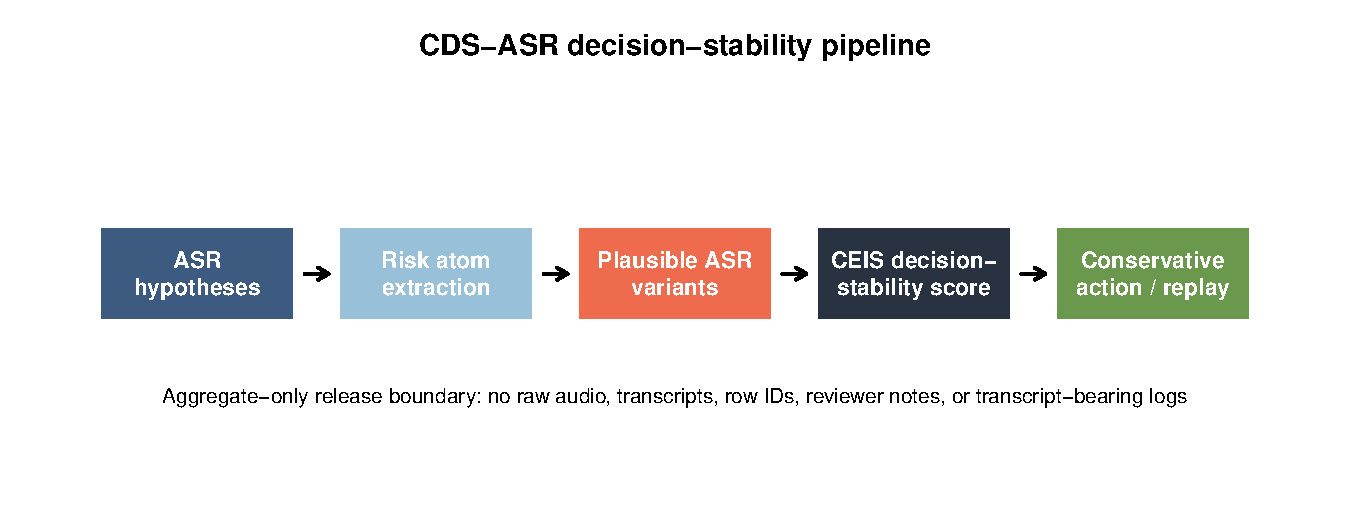
\includegraphics[width=\linewidth]{figures/fig1_pipeline.pdf}
\caption{CDS-ASR decision-stability pipeline. The figure is generated by \artifact{paper_4a_cds_asr/r/build_fig1_pipeline.R} from the manuscript protocol and aggregate method definitions.}
\label{fig:pipeline}
\end{figure}

The pipeline links transcript evidence to action evidence. ASR hypothesis generation creates transcript candidates and runtime signals. Risk-atom extraction identifies spoken spans whose alternatives can move the action boundary. Variant construction creates bounded alternatives from acoustic ambiguity, Mandarin phonetic and lexical confusions, domain-slot alternatives, model disagreement, and quality signals. Decision-instability scoring maps the original hypothesis and each variant through the declared action function. Aggregate policy replay evaluates how conservative operating rules respond to rows with elevated decision-instability evidence.

\subsection{Risk Atom Schema}

Risk atoms are spoken transcript spans that carry a direct decision role. The current schema includes negation, amount, actor, action, time, intent, uncertainty, and scam pattern. These atoms are selected because plausible ASR alternatives around them can move the declared safe action. The paper-facing schema below records the decision role of each atom class. The versioned configuration is \artifact{80_semantic_risk_asr/scoring/ceis_config.json}; the method summary is \artifact{70_experiments/runs/postdoc_evidence_chain_2026_05_25/ceis_method_summary.tsv}.

\begin{center}
\noindent\textbf{Risk atom schema for CDS-ASR.}

\begin{tabularx}{\linewidth}{@{}lL@{}}
\toprule
Risk atom & Decision relevance \\
\midrule
Negation & Can invert whether a transfer, contact, or authorization occurred. \\
Amount & Can change severity, priority, and escalation thresholds. \\
Actor & Can change who initiated or received the action. \\
Action & Can change whether the caller transferred, clicked, paid, reported, or refused. \\
Time & Can change urgency and incident sequence. \\
Intent & Can change whether a phrase is interpreted as request, refusal, uncertainty, or confirmation. \\
Uncertainty & Can change the appropriate review or abstention path. \\
Scam pattern & Can match or miss a known fraud scenario. \\
\bottomrule
\end{tabularx}
\end{center}


\subsection{Counterfactual Variant Contract}

The counterfactual variant contract converts recognition ambiguity into auditable decision-stability evidence. A valid variant is localized around a risk atom or supported by model disagreement and quality signals; it is acoustically or semantically plausible in Mandarin anti-fraud speech; and it is actionable enough to test the declared triage function. The construction draws from Mandarin phonetic and lexical confusions, amount and time slots, actor and action substitutions, negation and uncertainty alternatives, scam-pattern alternatives, and observed ASR disagreement. Public release reports aggregate coverage in \artifact{70_experiments/runs/janus_300_high_stakes_human_audit_selection_2026_05_25/counterfactual_variant_coverage_summary.tsv}.

\subsection{Downstream Decision Function}

The downstream decision function is a declared retrospective policy contract. It maps each transcript and variant to a triage action using the risk atoms visible in the text. The contract turns transcript alternatives into a policy-space representation that supports row-clustered analysis, decision-change labeling, and fixed-budget replay. The action space is operational by design: routine routing, manual review, priority review, critical escalation, conservative machine action, and abstention.

\subsection{CEIS}

CEIS is a bounded decision-instability score over plausible variants:
\[
\mathrm{CEIS}(x) = \max_{v \in V(x)} P_{\mathrm{plaus}}(v \mid x) \cdot W_{\mathrm{atom}}(v) \cdot D(d(\hat{t}), d(v)).
\]
Here $V(x)$ is the set of plausible variants, $P_{\mathrm{plaus}}$ is an audit-bounded plausibility score, $W_{\mathrm{atom}}$ is a risk-atom weight, and $D$ is a downstream decision-distance term. CEIS ranks each row by the strongest plausible movement from transcript evidence to action evidence. The score is interpretable by design: the three terms show why a row is decision-sensitive, which atom carries the action boundary, and how far the declared decision moves.

\subsection{Conservative-Action Policy Contract}

Aggregate policy replay evaluates five operating rules: baseline action, confidence-triggered review, SRES-triggered review, CEIS-triggered conservative action, and CEIS ensemble arbitration. Replay thresholds are retrospective diagnostic operating points on the scoped audit set. The replay layer connects method design to operational use by measuring how transcript accuracy, semantic-risk evidence, and counterfactual decision-stability evidence support conservative review allocation under a fixed budget.

\section{Experimental Setup}

\subsection{Evidence Layers}

The evidence design separates four layers: the 258-row ASR model-comparison split, selected-300 enriched high-stakes provenance outputs, a completed 300-row dual-reviewer human audit, and 900 model-level assessments per reviewer clustered within those 300 reviewed rows. Figure~\ref{fig:evidence_ladder} summarizes the design.

\begin{figure}[htbp]
\centering
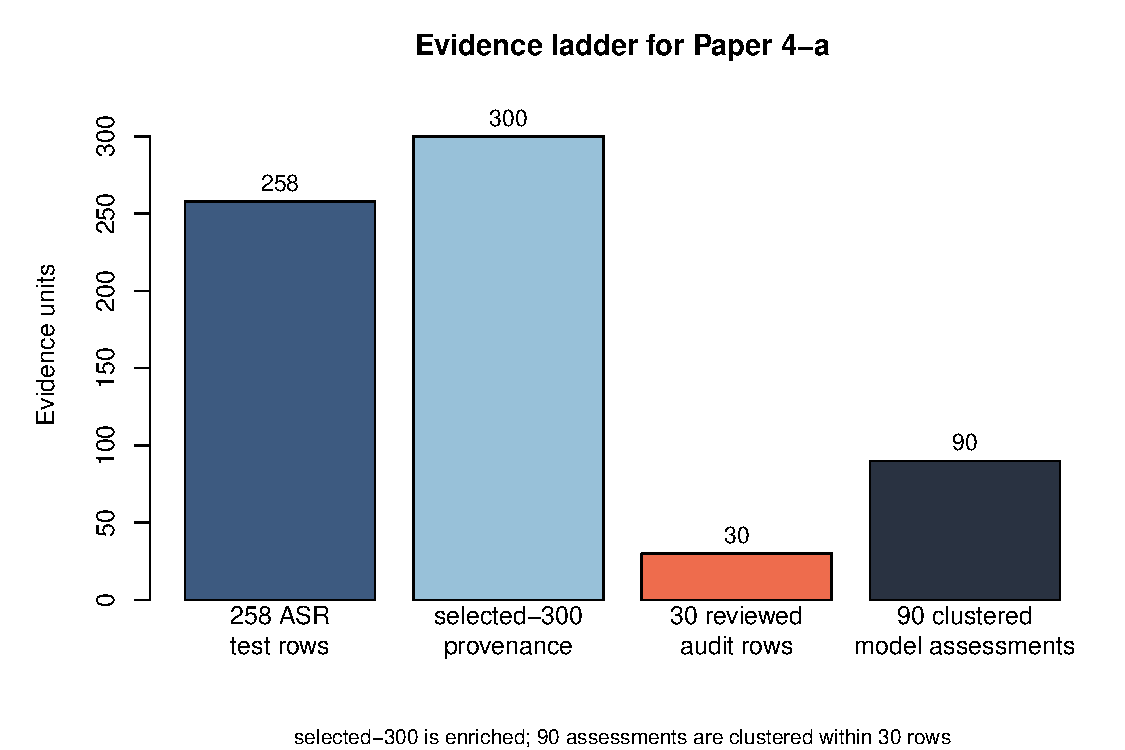
\includegraphics[width=.9\linewidth]{figures/fig2_evidence_ladder.pdf}
\caption{Evidence ladder for Paper 4-a. The figure is generated by \artifact{paper_4a_cds_asr/r/build_fig2_evidence_ladder.R} from aggregate evidence counts and the manuscript evidence boundary.}
\label{fig:evidence_ladder}
\end{figure}

The 258-row split provides ASR model-comparison context. The selected-300 layer is an enriched high-stakes audit surface and is not prevalence-preserving. The reviewed evidence layer consists of 300 rows per reviewer and 900 clustered model-level assessments per reviewer. The outcome label is human-reviewed decision change. Two reviewers completed the same selected-300 surface; Cohen's kappa is 0.849970 for decision-change labels, 1.000000 for semantic-risk labels, 0.851426 for expected safe action, and 0.934274 for annotation confidence. Reviewer agreement is treated as a validation layer over the same audit surface, while reviewer-specific labels are preserved separately for CEIS ablation rather than collapsed into an inferred adjudication.

\subsection{Baselines And Outcome}

The predictor comparison evaluates WER, CER, SRES, and CEIS against human-reviewed decision-change labels. WER and CER represent transcript-centered evidence, SRES represents semantic-risk evidence, and CEIS represents counterfactual decision-stability evidence.

\subsection{Uncertainty And Sensitivity}

Row-clustered uncertainty is reported from \artifact{70_experiments/runs/janus_300_high_stakes_human_audit_selection_2026_05_25/human_audit_predictor_clustered_ci.tsv}. Leave-one-row-out sensitivity is recorded in \artifact{70_experiments/runs/janus_300_high_stakes_human_audit_selection_2026_05_25/human_audit_predictor_leave_one_row_out.tsv}. Recovery-policy uncertainty and sensitivity are recorded in the corresponding aggregate recovery artifacts.

\subsection{CEIS Ablation Design}

The expanded dual-reviewer surface is used for an aggregate-only CEIS ablation. The variants are full CEIS, CEIS without atom weights, CEIS without plausibility, binary atom triggering, and top-3 mean aggregation over full CEIS components. The ablation isolates the mechanism that CDS-ASR contributes: decision-changing risk-atom instability under plausible alternatives. All ablation outputs are reviewer-separated aggregate summaries and exclude raw audio, transcripts, row identifiers, hypotheses, reviewer notes, and transcript-bearing merged sheets.

\section{Results}

\subsection{ASR Model-Comparison Context}

Table~\ref{tab:asr_benchmark} reports the 258-row ASR benchmark context. The partial-encoder run has the strongest current aggregate CER and WER profile in this split. This is model-comparison context only; it does not by itself establish downstream safety.

\begin{table}[htbp]
\centering
\caption{Main ASR benchmark on the 258-row split. Source: \artifact{70_experiments/runs/janus_258_test_split_asr_cds_proxy/asr_cds_proxy_comparison.tsv}.}
\label{tab:asr_benchmark}
\begin{tabular}{lrrrr}
\toprule
Run & Rows & CER zh micro & WER zh jieba micro & High-risk missed \\
\midrule
Partial encoder & 258 & 15.04 & 21.53 & 4 \\
LoRA legacy best & 258 & 18.23 & 25.59 & 7 \\
Breeze ASR25 base & 258 & 22.72 & 30.39 & 30 \\
Breeze ASR26 & 258 & 24.27 & 32.29 & 22 \\
\bottomrule
\end{tabular}
\end{table}


\subsection{Predictor Comparison}

Table~\ref{tab:predictor} and Figure~\ref{fig:predictor_auc} compare WER, CER, SRES, and CEIS against human-reviewed decision-change labels. CEIS has the strongest point AUC in the scoped audit and reaches a zero-false-negative diagnostic operating point. This is reported as a decision-stability signal under the selected audit boundary, not as a deployment threshold or universal classifier claim.

\begin{table}[htbp]
\centering
\caption{Predictor performance against human-reviewed decision-change labels. Source: \artifact{human_audit_predictor_comparison.tsv}. Thresholds are diagnostic operating points on the scoped audit set.}
\label{tab:predictor}
\begin{tabular}{lrrrrr}
\toprule
Metric & AUC & Best threshold & F1 & Recall & FN \\
\midrule
WER & 0.6964 & 42.59 & 0.4615 & 0.5625 & 7 \\
CER & 0.7276 & 16.42 & 0.4516 & 0.8750 & 2 \\
SRES & 0.8995 & 270.00 & 0.6512 & 0.8750 & 2 \\
CEIS & 0.9117 & 5.00 & 0.6275 & 1.0000 & 0 \\
\bottomrule
\end{tabular}
\end{table}


\begin{figure}[htbp]
\centering
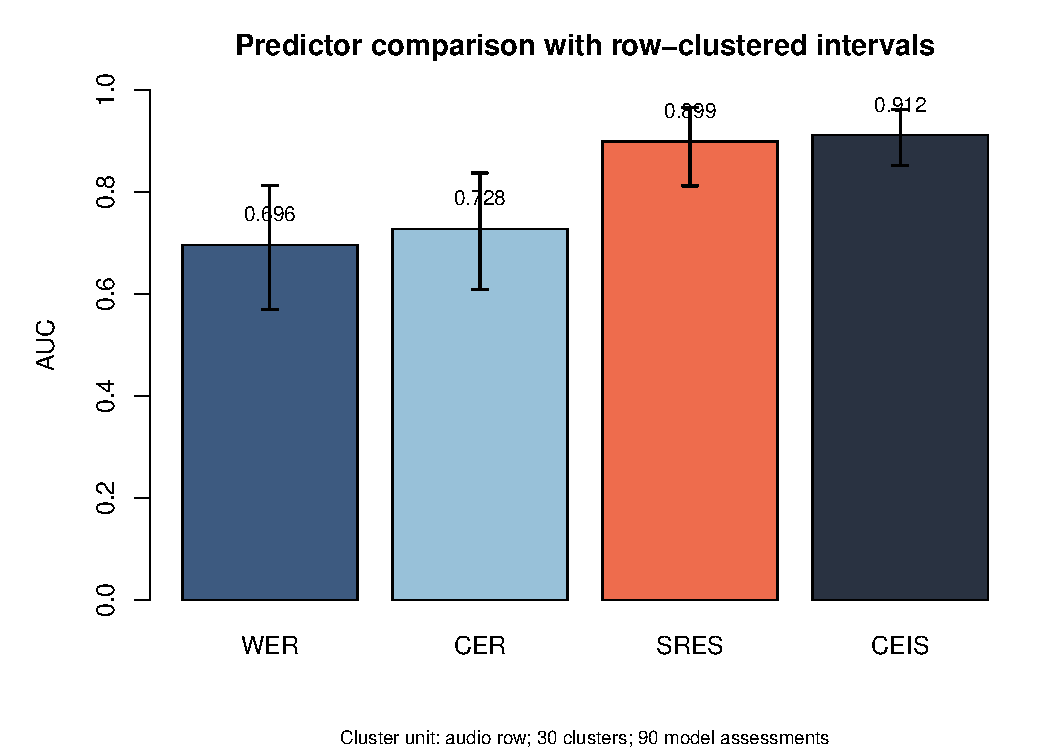
\includegraphics[width=.9\linewidth]{figures/fig3_predictor_auc.pdf}
\caption{Predictor comparison for WER, CER, SRES, and CEIS with row-clustered intervals. Source artifacts: \artifact{human_audit_predictor_comparison.tsv} and \artifact{human_audit_predictor_clustered_ci.tsv}.}
\label{fig:predictor_auc}
\end{figure}

\subsection{Aggregate Policy Replay}

Table~\ref{tab:policy} and Figure~\ref{fig:policy_replay} report aggregate policy replay. SRES-triggered recovery and CEIS-triggered conservative action eliminate high-risk missed and critical miss counts in aggregate replay at the same diagnostic budget. CEIS ensemble arbitration adds abstention behavior at a higher budget.

\begin{table}[htbp]
\centering
\caption{Aggregate policy replay under human-reviewed selected-300 labels. Source: \artifact{policy_comparison.tsv}.}
\label{tab:policy}
\small
\begin{tabularx}{\linewidth}{@{}Lrrrr@{}}
\toprule
Policy & Budget & Unsafe downrouting & High-risk missed & Critical miss \\
\midrule
No recovery & 0.0000 & 29 & 6 & 1 \\
Confidence only & 0.0000 & 29 & 6 & 1 \\
SRES recovery & 0.3889 & 24 & 0 & 0 \\
CEIS conservative action & 0.3889 & 24 & 0 & 0 \\
CEIS ensemble arbitration & 0.5222 & 24 & 0 & 0 \\
\bottomrule
\end{tabularx}
\end{table}


\begin{figure}[htbp]
\centering
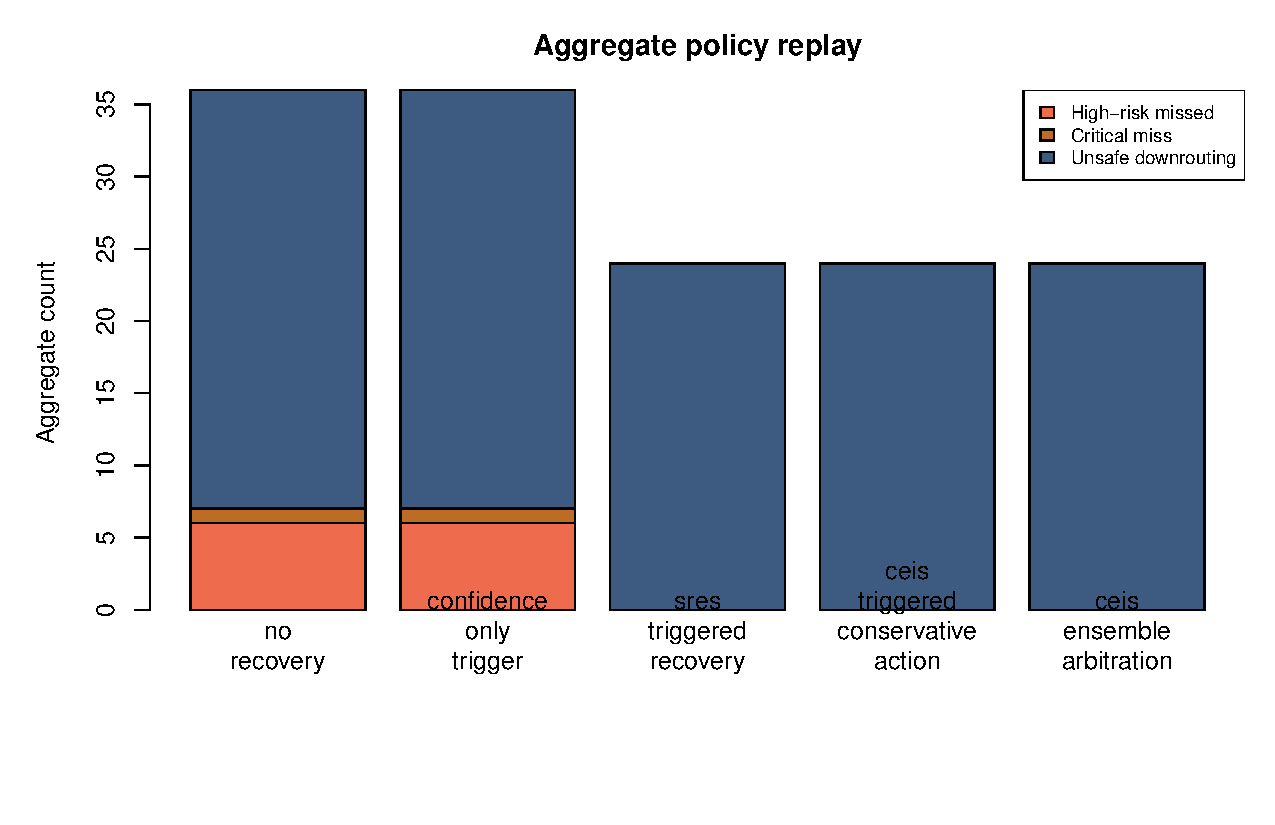
\includegraphics[width=.9\linewidth]{figures/fig4_policy_replay.pdf}
\caption{Aggregate policy replay under human-reviewed selected-300 labels. Source artifact: \artifact{70_experiments/runs/janus_300_high_stakes_recovery_human_reviewed_2026_05_26/policy_comparison.tsv}.}
\label{fig:policy_replay}
\end{figure}

\subsection{Fixed-Budget Frontier And Risk Atoms}

Figure~\ref{fig:frontier} shows the fixed-budget conservative replay frontier. Figure~\ref{fig:risk_atom} summarizes human-reviewed decision-change evidence by risk atom.

\begin{figure}[htbp]
\centering
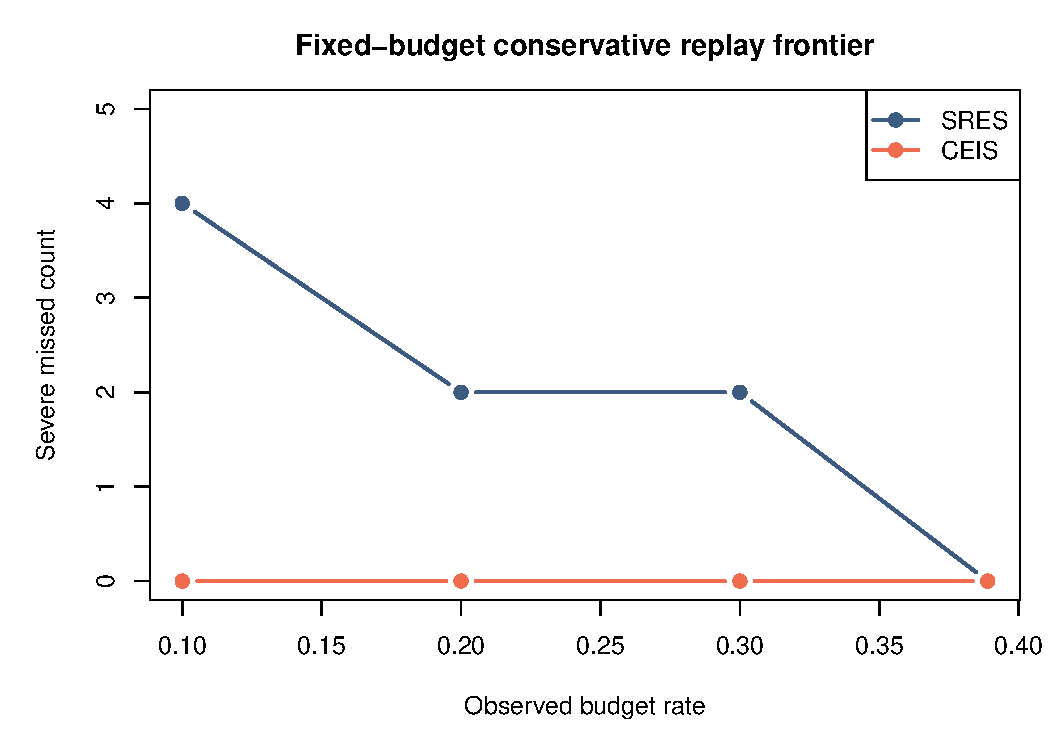
\includegraphics[width=.9\linewidth]{figures/fig5_fixed_budget_frontier.pdf}
\caption{Fixed-budget conservative replay frontier. Source artifact: \artifact{70_experiments/runs/janus_300_high_stakes_recovery_human_reviewed_2026_05_26/fixed_budget_recovery_frontier.tsv}.}
\label{fig:frontier}
\end{figure}

\begin{figure}[htbp]
\centering
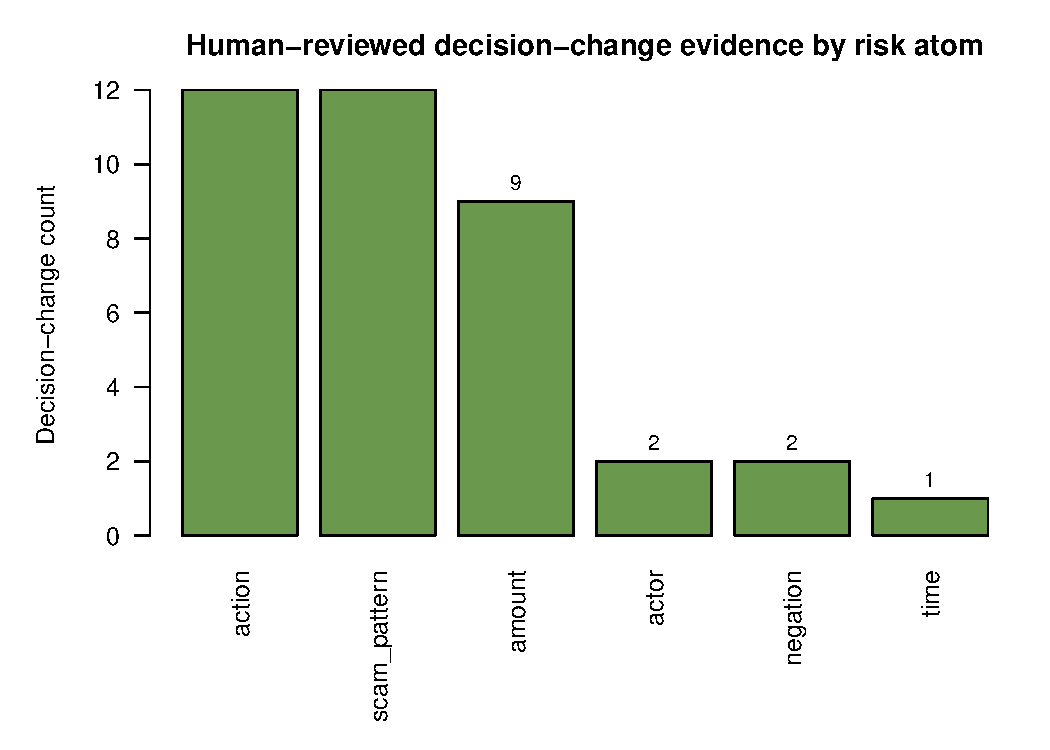
\includegraphics[width=.9\linewidth]{figures/fig6_risk_atom_review.pdf}
\caption{Human-reviewed decision-change evidence by risk atom. Source artifact: \artifact{70_experiments/runs/janus_300_high_stakes_human_audit_selection_2026_05_25/human_audit_risk_atom_review.tsv}.}
\label{fig:risk_atom}
\end{figure}

\section{Discussion}

The evidence supports a speech-evaluation claim: WER and CER remain necessary, but high-stakes speech-driven decision systems need an additional decision-stability layer. CEIS directly targets the question of whether plausible ASR alternatives around risk atoms would change downstream action.

CEIS should be interpreted conservatively. It is not a calibrated acoustic posterior and not a universal classifier. It is a decision-instability signal built from bounded plausible variants, risk-atom weighting, and downstream decision distance. In the current scoped audit, CEIS has the strongest point AUC and a zero-false-negative diagnostic operating point, while SRES remains a strong semantic-risk baseline.

Better ASR models reduce transcript error but do not remove the need for downstream decision-stability analysis. The model-comparison split identifies the strongest current hypothesis generator; the human-reviewed audit tests whether remaining uncertainty affects decisions.

\section{Limitations And Ethics}

The reviewed audit is small in the current draft: 30 human-reviewed rows and 90 model-row assessments clustered within those rows. The 90 assessments are not 90 independent calls. Human review is a single-expert pilot audit; no inter-annotator agreement is claimed in the current draft. The submission-validation plan expands the audit to 100+ completed rows, adds a second reviewer, and reports Cohen's kappa or Fleiss' kappa before submission. The selected-300 layer is an enriched high-stakes audit surface, not a prevalence-preserving sample.

Thresholds are diagnostic operating points on the scoped audit set. They are not frozen deployment thresholds. Aggregate replay is retrospective and does not establish live deployment readiness or population prevalence of ASR-induced harm.

Raw audio, raw transcripts, selected row identifiers, reviewer notes, and transcript-bearing runtime logs remain outside the public release boundary. The intended use is ASR safety audit, review prioritization, conservative escalation, and abstention. CDS-ASR is not proposed for automatic punitive action, account restriction, guilt determination, or direct law-enforcement reporting without human review.

\appendix
\section{Appendix: Aggregate Artifacts And Submission Notes}

The appendix records the aggregate artifacts used by the manuscript. Long operation records, validation gate commands, candidate-lane details, and full claim registries are moved out of the main text to keep Paper 4-a speech-centered.

\begin{itemize}
\item ASR split comparison: \artifact{70_experiments/runs/janus_258_test_split_asr_cds_proxy/asr_cds_proxy_comparison.tsv}
\item Predictor comparison: \artifact{70_experiments/runs/janus_300_high_stakes_human_audit_selection_2026_05_25/human_audit_predictor_comparison.tsv}
\item Predictor clustered CI: \artifact{70_experiments/runs/janus_300_high_stakes_human_audit_selection_2026_05_25/human_audit_predictor_clustered_ci.tsv}
\item Recovery replay: \artifact{70_experiments/runs/janus_300_high_stakes_recovery_human_reviewed_2026_05_26/policy_comparison.tsv}
\item Fixed-budget frontier: \artifact{70_experiments/runs/janus_300_high_stakes_recovery_human_reviewed_2026_05_26/fixed_budget_recovery_frontier.tsv}
\item Risk atom review: \artifact{70_experiments/runs/janus_300_high_stakes_human_audit_selection_2026_05_25/human_audit_risk_atom_review.tsv}
\item Completed dual-reviewer audit record: \artifact{70_experiments/runs/janus_300_high_stakes_human_audit_completed_300_dual_reviewer_2026_06_02/}
\item CEIS ablation summary: \artifact{70_experiments/runs/janus_300_high_stakes_ceis_ablation_dual_reviewer_2026_06_02/}
\item CEIS method summary: \artifact{70_experiments/runs/postdoc_evidence_chain_2026_05_25/ceis_method_summary.tsv}
\item Artifact manifest: \artifact{80_semantic_risk_asr/paper/artifact_manifest.tsv}
\end{itemize}

\section{Ablation Status}

Aggregate-safe CEIS ablation is complete on the selected-300 dual-reviewer surface. The tracked output folder contains \artifact{ceis_ablation_summary.json}, \artifact{ceis_ablation_predictor_summary.tsv}, \artifact{ceis_ablation_policy_replay.tsv}, \artifact{ceis_ablation_model_summary.tsv}, \artifact{ceis_ablation_delta_summary.tsv}, and an interpretation note. These outputs are aggregate-only and exclude transcript-bearing reviewer sheets, merged sheets, raw audio, raw transcripts, row identifiers, reviewer notes, and completed review packages.


\bibliographystyle{unsrtnat}
\bibliography{references}

\end{document}
